\section{Proyek -- Sistem Deteksi Gas \& Penanganan Darurat Otomatis}
\label{sec:proyek-eksperimen}

Proyek ini dirancang untuk menguji integrasi multikomponen berbasis interupsi eksternal dan kontrol non-pemblokiran (\textit{non-blocking}) pada mikrokontroler Arduino Mega 2560. Sistem menggabungkan logika operasional harian (akses pintu otomatis berbasis gerakan) dan logika penanganan darurat prioritas tinggi (mitigasi kebocoran gas).
\subsection{Desain Sistem}
\label{subsec:desain_sistem}

Sistem keselamatan ini dirancang menggunakan arsitektur dual-mode berbasis prioritas pemrosesan: \textbf{Mode Reguler} (manajemen akses pintu otomatis berbasis deteksi gerakan) dan \textbf{Mode Darurat} (mitigasi kebocoran gas berbasis interupsi eksternal \textit{hardware}).

Interkoneksi fisik dan alokasi pin antarmuka mikrokontroler Arduino Mega 2560 disajikan secara terisolasi pada Gambar~\ref{fig:blok_simpel}.

\begin{figure}[htbp]
	\centering
	\begin{tikzpicture}[
			node distance=1.5cm and 1.5cm,
			blok/.style={draw, rectangle, rounded corners=3pt, minimum width=2.8cm, minimum height=1.0cm, align=center, font=\sffamily\small, fill=blue!6, line width=0.8pt},
			mcu/.style={draw, rectangle, rounded corners=4pt, minimum width=3.2cm, minimum height=2.4cm, align=center, font=\sffamily\small, fill=teal!10, line width=1.2pt},
			panah/.style={->, >=stealth, thick, line width=0.9pt}
		]
		% Node Input (Kiri)
		\node[blok] (gas) {Sensor Gas};
		\node[blok, below=0.8cm of gas] (pir) {Sensor PIR};

		% Node MCU (Tengah)
		\node[mcu, right=1.5cm of gas, yshift=-0.9cm] (mcu) {\textbf{Arduino Mega 2560}};

		% Node Output (Kanan)
		\node[blok, right=1.5cm of mcu, yshift=0.9cm] (relay) {Modul Relai};
		\node[blok, below=0.8cm of relay] (servo) {Micro Servo};

		% Garis Penghubung Input ke MCU
		\draw[panah, color=red!70!black] (gas.east) -- node[above, font=\tiny\sffamily, color=black] {Pin 2 (\texttt{INT0})} (gas.east -| mcu.west);
		\draw[panah] (pir.east) -- node[above, font=\tiny\sffamily, color=black] {Pin 8} (pir.east -| mcu.west);

		% Garis Penghubung MCU ke Output
		\draw[panah, color=red!70!black] (mcu.east |- relay.west) -- node[above, font=\tiny\sffamily, color=black] {Pin 3} (relay.west);
		\draw[panah] (mcu.east |- servo.west) -- node[above, font=\tiny\sffamily, color=black] {Pin 9 (\texttt{PWM})} (servo.west);
	\end{tikzpicture}
	\caption{Diagram blok antarmuka periferal dan aktuator sistem.}
	\label{fig:blok_simpel}
\end{figure}

Alur eksekusi logika dipisahkan secara tegas berdasarkan status atmosferik lingkungan:

\begin{enumerate}
	\item \textbf{Alur Operasi Normal (PIR \& Pintu Otomatis):} Pada kondisi aman, mikrokontroler mengeksekusi \textit{polling} non-pemblokiran (\textit{non-blocking}) memanfaatkan pewaktu internal \texttt{millis()}. Jika sensor PIR mendeteksi gerakan (logika \texttt{HIGH}), \textit{servo motor} bergerak ke sudut $140^\circ$. Pintu akan dipertahankan terbuka selama penunda waktu (\textit{hold time}) minimal $1000\,\text{ms}$ sebelum ditutup kembali ke sudut $45^\circ$.
	\item \textbf{Alur Penanganan Darurat (Interupsi Kebocoran Gas):} Saat sensor gas mendeteksi kebocoran, keluaran digital berubah menjadi \texttt{LOW} (\textit{Active-LOW}) dan langsung memicu interupsi \texttt{INT0} pada pemicuan tepi turun (\textit{FALLING edge}). Rutin \textit{Interrupt Service Routine} (ISR) mengesampingkan eksekusi normal, mengaktifkan kipas pembuang udara melalui modul relai (Pin 3 \texttt{HIGH}), serta mematikan dan mengunci posisi pintu servo pada sudut $45^\circ$ hingga udara dinyatakan aman.
\end{enumerate}

Diagram alur (\textit{flowchart}) untuk kedua mode operasional disajikan secara bersandingan menggunakan \textit{subfigure} pada Gambar~\ref{fig:flowcharts_side_by_side}.

\begin{figure}[htbp]
	\centering
	% ------------------ SUBFIGURE 1: ALUR NORMAL (KIRI) ------------------
	\begin{subfigure}[t]{0.49\textwidth}
		\centering
		\begin{tikzpicture}[
				node distance=0.6cm,
				startend/.style={draw, rectangle, rounded corners=8pt, minimum width=2.4cm, minimum height=0.6cm, align=center, font=\sffamily\scriptsize, fill=gray!15, line width=0.6pt},
				proses/.style={draw, rectangle, minimum width=2.8cm, minimum height=0.6cm, align=center, font=\sffamily\scriptsize, fill=blue!5, line width=0.6pt},
				keputusan/.style={draw, diamond, aspect=2, minimum width=2.6cm, minimum height=0.7cm, align=center, font=\sffamily\scriptsize, fill=orange!10, line width=0.6pt},
				panah/.style={->, >=stealth, semithick}
			]
			\node[startend] (start) {Mulai Loop Normal};
			\node[proses, below=of start] (read) {Baca Status Pin PIR};
			\node[keputusan, below=of read] (cek_pir) {PIR == HIGH?};
			\node[proses, below=of cek_pir] (buka) {Buka Servo ($140^\circ$)\\Catat \texttt{openStartTime}};
			\node[keputusan, below=of buka] (cek_timer) {Timer $\ge 1000\,\text{ms}$?};
			\node[proses, below=of cek_timer] (tutup) {Tutup Servo ($45^\circ$)\\Status \texttt{isOpen} = false};
			\node[startend, below=of tutup] (end) {Selesai Iterasi};

			% Garis Alur Utama
			\draw[panah] (start) -- (read);
			\draw[panah] (read) -- (cek_pir);
			\draw[panah] (cek_pir) -- node[right, font=\scriptsize] {Ya} (buka);
			\draw[panah] (buka) -- (cek_timer);
			\draw[panah] (cek_timer) -- node[right, font=\scriptsize] {Ya} (tutup);
			\draw[panah] (tutup) -- (end);

			% Garis Bypass (Tidak)
			\draw[panah] (cek_pir.east) -- ++(0.5,0) |- node[near start, right, font=\scriptsize] {Tidak} (cek_timer.east);
			\draw[panah] (cek_timer.west) -- ++(-0.5,0) |- node[near start, left, font=\scriptsize] {Tidak} (end.west);
		\end{tikzpicture}
		\caption{Mode reguler (PIR \& Servo).}
		\label{fig:flowchart_normal_sub}
	\end{subfigure}
	\hfill
	% ------------------ SUBFIGURE 2: ALUR DARURAT (KANAN) ------------------
	\begin{subfigure}[t]{0.49\textwidth}
		\centering
		\begin{tikzpicture}[
				node distance=0.6cm,
				startend/.style={draw, rectangle, rounded corners=8pt, minimum width=2.4cm, minimum height=0.6cm, align=center, font=\sffamily\scriptsize, fill=red!15, line width=0.6pt},
				proses/.style={draw, rectangle, minimum width=2.8cm, minimum height=0.6cm, align=center, font=\sffamily\scriptsize, fill=red!5, line width=0.6pt},
				keputusan/.style={draw, diamond, aspect=2, minimum width=2.6cm, minimum height=0.7cm, align=center, font=\sffamily\scriptsize, fill=orange!10, line width=0.6pt},
				panah/.style={->, >=stealth, semithick}
			]
			\node[startend] (start) {Interupsi Gas Terpemicu};
			\node[proses, below=of start] (flag) {Set \texttt{emergencyFlag} = true};
			\node[proses, below=of flag] (action) {1. Detach Interupsi\\2. Relai Kipas HIGH\\3. Servo Tutup ($45^\circ$)};
			\node[keputusan, below=of action] (cek_gas) {Pin Gas == LOW?};
			\node[proses, below=of cek_gas] (clear) {1. Relai Kipas LOW\\2. Reset \texttt{emergencyFlag}\\3. Attach Interupsi};
			\node[startend, below=of clear] (end) {Kembali Mode Normal};

			% Garis Alur Utama
			\draw[panah] (start) -- (flag);
			\draw[panah] (flag) -- (action);
			\draw[panah] (action) -- (cek_gas);
			\draw[panah] (cek_gas) -- node[right, font=\scriptsize] {Tidak (Aman)} (clear);
			\draw[panah] (clear) -- (end);

			% Garis Loop Kondisi Masih Ada Gas (Ya)
			\draw[panah] (cek_gas.west) -- ++(-0.5,0) |- node[near start, left, font=\scriptsize] {Ya} (action.west);
		\end{tikzpicture}
		\caption{Mode darurat (Interupsi Gas).}
		\label{fig:flowchart_emergency_sub}
	\end{subfigure}
	\caption{Diagram alur logika eksekusi sistem: (a) Mode operasional harian berbasis PIR dan (b) Mode penanganan kebocoran gas berbasis interupsi.}
	\label{fig:flowcharts_side_by_side}
\end{figure}

\subsection{Rangkaian dan Koneksi}
Pemetaan koneksi fisik antara komponen antarmuka dan mikrokontroler Arduino Mega 2560 dirangkum pada Tabel~\ref{tab:koneksi_proyek}.

\begin{figure}[htbp]
	\centering
	% Ganti dengan file skematik rangkaian aktual atau tangkapan layar simulasi Wokwi
	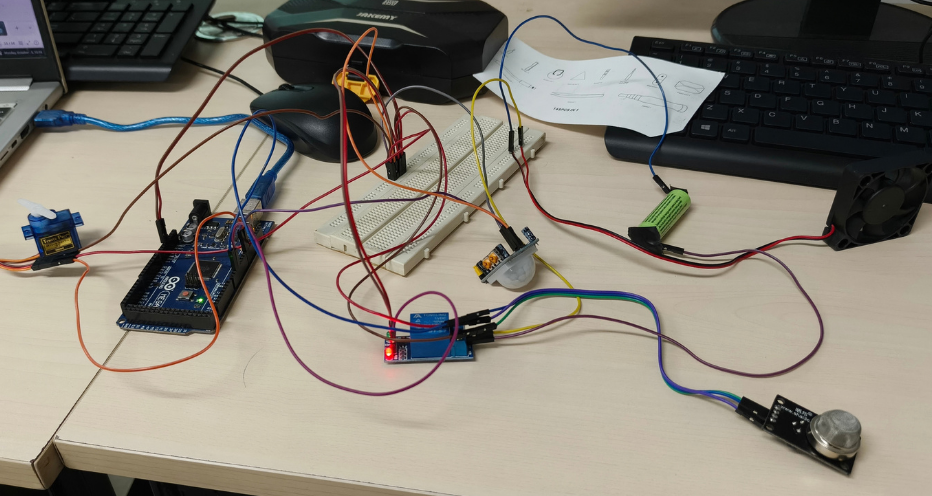
\includegraphics[width=0.70\textwidth]{images/rangkaian_proyek.png}
	% \fbox{\parbox[c][5cm][c]{0.70\textwidth}{\centering Tempatkan tangkapan layar simulasi Wokwi atau diagram skematik antarmuka Sensor MQ dengan Arduino Mega 2560 di sini}}
	\caption{Rangkaian Sistem Deteksi Gas \& Penanganan Darurat Otomatis.}
	\label{fig:rangkaian_sistem}
\end{figure}



\begin{table}[H]
	\centering
	\caption{Pemetaan antarmuka komponen ke Arduino Mega 2560}
	\label{tab:koneksi_proyek}
	\small
	\begin{tabularx}{\textwidth}{@{} p{3.2cm} p{3.8cm} X @{}}
		\toprule
		Komponen          & Pin MCU                       & Alasan Pemilihan \& Fungsi                                                             \\
		\midrule
		Sensor Gas (DOUT) & Pin Digital 2 (\texttt{INT0}) & Mendukung fitur interupsi eksternal hardware untuk deteksi kebocoran gas secara instan \\
		Sensor PIR (OUT)  & Pin Digital 8                 & Membaca logika keberadaan objek untuk aktuasi pintu otomatis                           \\
		Modul Relai (IN)  & Pin Digital 3                 & Sakelar daya beban induktif kipas eksternal                                            \\
		Servo Motor (PWM) & Pin Digital 9                 & Mengendalikan sudut bukaan engsel pintu otomatis ($45^\circ\text{--}140^\circ$)        \\
		\bottomrule
	\end{tabularx}
\end{table}

\subsection{Program Eksperimen}
Kode program diimplementasikan menggunakan arsitektur \textit{state machine} sederhana yang mengisolasi eksekusi mode reguler dan mode darurat melalui bendera interupsi \textit{volatile} (\texttt{emergencyFlag}).

\begin{lstlisting}[language=C++, caption={Kode program sistem deteksi gas dan penanganan darurat otomatis}, label={lst:proyek_code}]
#include <Servo.h>

const int GAS_PIN = 2;
const int RELAY_PIN = 3;
const int PIR_PIN = 8;
const int SERVO_PIN = 9;

const int SERVO_CLOSED_ANGLE = 45;
const int SERVO_OPEN_ANGLE = 140;

Servo myServo;
volatile bool emergencyFlag = false;

unsigned long openStartTime = 0;
bool isOpen = false;
const unsigned long HOLD_TIME = 1000;

void gasDetectedISR() {
  if (digitalRead(GAS_PIN) == LOW) {
    emergencyFlag = true;
  }
}

void setup() {
  Serial.begin(9600);

  pinMode(GAS_PIN, INPUT);
  pinMode(RELAY_PIN, OUTPUT);
  pinMode(PIR_PIN, INPUT);

  digitalWrite(RELAY_PIN, LOW);

  myServo.attach(SERVO_PIN);
  myServo.write(SERVO_CLOSED_ANGLE);

  attachInterrupt(digitalPinToInterrupt(GAS_PIN), gasDetectedISR, FALLING);

  Serial.println("System Initialized. Running normal PIR + Servo loop...");
}

void loop() {
  if (emergencyFlag) {
    runEmergencyLoop();
  } else {
    runRegularLoop();
  }
}

void runRegularLoop() {
  int pirState = digitalRead(PIR_PIN);
  unsigned long currentMillis = millis();

  if (pirState == HIGH && !isOpen) {
    Serial.println("Motion detected! Opening servo...");
    myServo.write(SERVO_OPEN_ANGLE);
    isOpen = true;
    openStartTime = currentMillis;
  }

  if (isOpen && (currentMillis - openStartTime >= HOLD_TIME)) {
    if (pirState == LOW) {
      Serial.println("Motion cleared. Closing servo...");
      myServo.write(SERVO_CLOSED_ANGLE);
      isOpen = false;
    } else {
      openStartTime = currentMillis;
    }
  }

  delay(50);
}

void runEmergencyLoop() {
  detachInterrupt(digitalPinToInterrupt(GAS_PIN));

  Serial.println("EMERGENCY ALERT: Gas detected! Activating relay.");
  digitalWrite(RELAY_PIN, HIGH);
  myServo.write(SERVO_CLOSED_ANGLE);
  isOpen = false;

  while (digitalRead(GAS_PIN) == LOW) {
    Serial.println("WARNING: Gas levels still high. Holding emergency state...");
    delay(1000);
  }

  Serial.println("Gas cleared. Deactivating relay and resuming normal operation.");
  digitalWrite(RELAY_PIN, LOW);
  emergencyFlag = false;

  delay(100);
  attachInterrupt(digitalPinToInterrupt(GAS_PIN), gasDetectedISR, FALLING);
}
\end{lstlisting}

\subsection{Prosedur Pengujian Sistem}
Pengujian dilakukan untuk memvalidasi dua skenario operasional sistem:
\begin{enumerate}
	\item \textbf{Pengujian Mode Reguler (Otomatisasi Pintu):} Lakukan gerakan di depan sensor PIR saat kondisi udara normal (tidak ada indikasi kebocoran gas). Amati pergerakan \textit{servo motor} dari sudut $45^\circ$ ke $140^\circ$ serta penghitungan pewaktuan penutupan kembali setelah durasi penunda (\textit{hold time}) minimal $1000\,\text{ms}$ terpenuhi tanpa adanya presensi objek baru.
	\item \textbf{Pengujian Mode Darurat (Interupsi Kebocoran Gas):} Simulasi kondisi kebocoran gas dilakukan dengan memutar potensiometer bawaan pada modul sensor gas untuk menurunkan nilai ambang batas sensitivitas komparator hingga menguji pemicuan sinyal digital (\textit{digital output}). Saat mode reguler sedang berjalan, penyesuaian potensiometer ini akan mengubah sinyal keluaran sensor dari \texttt{HIGH} menjadi \texttt{LOW} (\textit{Active-LOW}). Amati transisi seketika sistem yang mengeksekusi \textit{Interrupt Service Routine} (ISR) menuju fungsi \texttt{runEmergencyLoop()}, penyaluran daya relai kipas pembuang udara, penguncian posisi servo pada sudut $45^\circ$, serta pemertahanan status darurat hingga potensiometer dikembalikan ke posisi semula (\textit{GAS\_PIN} kembali \texttt{HIGH}).
\end{enumerate}

\subsection{Analisis Hasil}
Hasil eksperimen menunjukkan bahwa penggunaan interupsi eksternal hardware pemicuan tepi turun (\textit{FALLING edge}) pada Pin 2 berhasil memberikan kepastian respons waktu nyata (\textit{real-time}) tanpa terhalang oleh siklus jeda \texttt{delay()} pada operasi reguler.

Penggunaan teknik \textit{timer} non-pemblokiran \texttt{millis()} pada fungsi \texttt{runRegularLoop()} menjamin ketersediaan waktu pemrosesan MCU yang tinggi. Saat kondisi darurat terdeteksi, pelepasan sementara interupsi (\texttt{detachInterrupt()}) di dalam \texttt{runEmergencyLoop()} secara efektif mencegah terjadinya pemicuan interupsi berulang (\textit{nesting interrupt}) selama kebocoran gas masih berlangsung.

\subsection{Validasi Pemahaman}
\begin{enumerate}
	\item \textbf{Mengapa komponen menghasilkan sinyal seperti yang diamati?}
	      Masing-masing komponen sensor menghasilkan karakteristik sinyal kontrol digital yang spesifik berdasarkan mekanisme pembacaannya:
	      \begin{itemize}
		      \item \textbf{Sinyal Terinterupsi Sensor Gas (Digital Output):} Modul sensor gas memanfaatkan komparator LM393 untuk membandingkan tegangan sensor analog dengan tegangan acuan potensiometer. Saat konsentrasi gas melebihi \textit{threshold}, komparator menarik saluran keluaran menjadi logika \texttt{LOW} ($0\,\text{V}$, \textit{Active-LOW}). Transisi tepi turun (\textit{FALLING edge}) dari $5\,\text{V}$ ke $0\,\text{V}$ ini menghasilkan sinyal interupsi \textit{hardware} instant pada pin \texttt{INT0}.
		      \item \textbf{Sinyal Polling Sensor PIR (Digital Output):} Pirosensor memproses perubahan radiasi inframerah termal dari objek bergerak melalui lensa Fresnel. Saat terjadi pergerakan, sirkuit pemroses internal memicu sinyal logika \texttt{HIGH} ($5\,\text{V}$, \textit{Active-HIGH}) yang dipertahankan selama durasi penunda (\textit{delay time}) bawaan modul.
	      \end{itemize}

	\item \textbf{Bagaimana perubahan input memengaruhi output?}
	      Sinyal kontrol input secara langsung memodelkan tingkah laku sinyal kontrol output berdasarkan prioritas logika:
	      \begin{itemize}
		      \item \textbf{Pengondisian Sinyal Normal (PIR ke Servo):} Penerimaan sinyal pemicu \texttt{HIGH} dari sensor PIR menginstruksikan modulasi lebar pulsa (\textit{Pulse Width Modulation}/PWM) pada Pin 9 untuk mengubah lebar pulsa \textit{duty cycle} dari $0{,}5\,\text{ms}$ (sudut tertutup $45^\circ$) menjadi $1{,}5\,\text{ms}$ (sudut terbuka $140^\circ$). Sinyal PWM ini dipertahankan hingga fungsi pewaktu \texttt{millis()} menyelesaikan kalkulasi penundaan $1000\,\text{ms}$.
		      \item \textbf{Pengondisian Sinyal Darurat (Gas ke Relai dan Servo):} Kemunculan sinyal \texttt{LOW} pada pin interupsi gas mengesampingkan (\textit{override}) seluruh sinyal logika PIR. Sinyal kontrol pemicu relai pada Pin 3 diubah menjadi logika \texttt{HIGH} untuk menyalakan kipas pembuang udara $6\,\text{V}$, secara bersamaan sinyal PWM Servo dipaksa kembali ke \textit{duty cycle} $0{,}5\,\text{ms}$ (sudut $45^\circ$) untuk mengunci posisi pintu.
	      \end{itemize}

	\item \textbf{Fitur mikrokontroler apa yang digunakan dan mengapa?}
	      Sistem mengalokasikan periferal mikrokontroler berdasarkan karakteristik sinyal kontrol yang dibutuhkan:
	      \begin{itemize}
		      \item \textbf{Interupsi Hardware Eksternal (\texttt{INT0}):} Digunakan khusus untuk mengawasi sinyal digital sensor gas. Fitur ini memungkinkan mikrokontroler untuk merespons transisi sinyal secara \textit{real-time} tanpa terhalang oleh eksekusi siklus program utama.
		      \item \textbf{Hardware Timer PWM (\texttt{Timer1}):} Digunakan untuk menghasilkan sinyal kontrol pulsa gelombang kotak berkala dengan frekuensi $50\,\text{Hz}$ untuk pengemudikan posisi poros \textit{servo motor} secara presisi.
		      \item \textbf{Pewaktu Sistem (\texttt{millis}):} Digunakan untuk manajemen pewaktuan sinyal kontrol PIR secara non-pemblokiran (\textit{non-blocking}), menjaga ketersediaan waktu eksekusi CPU tetap tinggi.
	      \end{itemize}

	\item \textbf{Bagian rangkaian mana yang paling menentukan perilaku sistem?}
	      Jalur sinyal logika interupsi pada Pin Digital 2 (\texttt{INT0}) dan variabel penanda \texttt{volatile bool emergencyFlag} merupakan elemen penentu utama perilaku sistem. Jalur ini bertindak sebagai sakelar logika tingkat tinggi yang mampu mengalihkan status sistem dari pengondisian sinyal reguler berbasis \textit{polling} menuju pengondisian sinyal tanggap darurat secara instan.
\end{enumerate}

\subsection{Kesimpulan}
Eksperimen sistem keselamatan ini berhasil mengintegrasikan sensor logika biner, sensor terinterupsi, \textit{servo motor}, dan modul sakelar relai daya. Penggunaan mekanisme interupsi eksternal terbukti efektif menjamin waktu tanggap darurat yang efisien, sementara penggunaan struktur kode non-pemblokiran menjaga kelancaran operasi rutin harian. Keterbatasan sistem ini terletak pada penggunaan sinyal digital sensor gas yang belum menyajikan nilai konsentrasi kuantitatif (PPM). Pengembangan selanjutnya dapat memanfaatkan pembacaan pin analog ADC serta penambahan indikator peringatan suara (\textit{buzzer}).
